\documentclass[11pt]{article}
\usepackage{amsmath,amssymb, amsthm, marvosym, permute, extsizes}
\usepackage{siunitx, graphicx, float, enumitem, adjustbox, hyperref, bm}
\usepackage{microtype, dsfont}
\usepackage[normalem]{ulem}
\usepackage{braket}
\usepackage[T1]{fontenc}
\usepackage[utf8]{inputenc}
\usepackage[justification=centering]{caption}
\usepackage{lmodern}
\usepackage[T1]{fontenc}
\usepackage[a4paper,margin=2.5cm]{geometry}
\usepackage[icelandic]{babel}
\usepackage{tikz}
\newcommand{\explain}[2]{\underbrace{#1}_\textrm{$#2$}}
\usepackage{minted}
\usemintedstyle{perldoc}
\parindent = 0pt
\usepackage{fancyhdr}
    \pagestyle{fancy}
    \headheight=32pt
    \lhead{Háskóli Íslands\\Raunvísindadeild}
    \rhead{Verkleg Eðlisfræði}
\title{{\Huge Þurrgufun Joðs}}
\author{Emil Gauti Friðriksson og Garðar Árni Skarphéðinsson}
\date{Janúar 2019 \\
\vspace{5cm}

\includegraphics[width = .6\textwidth]{HIlogo1.png}}

\begin{document}

\maketitle
\thispagestyle{empty}

\newpage

\section{Inngangur}
Varmafræðilegri hegðun efna má lýsa með bæði varmafræði og með safneðlisfræði. Hér verður fjallað um fasajafnvægi joðs við þurrgufun, $I_2(s) = I_2(g)$, og líkön byggð á báðum fræðunum borin saman við mældar niðurstöður. \\

\section{Líkan}
Þegar jafnvægi er á milli gasfasa og fasts kristalfasa er efnamætti fasanna einnig í jafnvægi, þ.e.

\begin{align}
\mu_s(T) = \mu_g(T)
\end{align}

Með safneðlisfræðilegum líkönum fást kórsummur fasanna tveggja og frá þeim fást efnamættin:

\begin{align}
\mu_s(T) = \frac{RT}{2} \left[\displaystyle\prod_{j=1}^{12} (1 - e^{-\Theta_j/T}) \right],
\end{align}

\begin{align}
\mu_g(T) = \Delta E_0^0 - RT\ln\left[\left(\frac{2\pi mkT}{h^2}\right)^{3/2} \frac{kT}{p}\frac{T}{\sigma\Theta_{rot}} (1 - e^{-\Theta_{vib}/T})^{-1} \right]
\end{align}

Nákvæmari útleiðslur má finna í vinnuseðli. Stærðirnar í jöfnunum að ofan eru eftirfarandi:\\
\begin{align}
\Theta_j = \frac{h\nu_j}{k}, \quad \Theta_{rot} = \frac{hcB_0}{k}, \quad \Theta_{vib} = \Theta_{j=0} \label{eq:theta}
\end{align}
$T:$ Hitastig\\
$p:$ Hlutþrýstingur\\
$c:$ Hraði  í lofttæmi\\
$h:$ Fasti Plancks\\
$k:$ Fasti Boltzmanns\\
$R:$ Gasfastinn\\
$\nu_j:$ Titringstíðni $I_2$ sameindar\\
$\Delta \widetilde{E}_0^0:$ Uppgufunarorka per mól\\
$m:$ Massi sameindar\\
$B_0:$ Snúningsfasti\\
$\sigma:$ Samhverfutala, $\sigma = 2$.\\
\\

Athugum nú tvær leiðir til þess að ákvarða uppgufunarvarma joðsins, $\Delta \widetilde{H}_{sub}$. Sú fyrri er með því að bera saman mældan þrýsting og hitastig við Clausius-Clapeyron venslin $\ln(p) = C - \Delta \widetilde{H}_{sub}/RT$, þar sem C er fasti. Besta lína grafs $\ln(p)$ sem fall af $1/T$ myndi þá hafa hallatölu $\Delta \widetilde{H}_{sub}/R$. Athugum að þrýsting má ákvarða út frá ljósgleypni joðsins, $A$, með jöfnunni:

\begin{align}
p = \frac{RTA}{d\epsilon}
\end{align}

Þar sem $\epsilon$ er mólar gleypnistuðull joðs og $d$ er breiddin sem afmarkar hreyfingu gassins, þ.e. breidd íláts.

\\
Önnur aðferð til þess að ákvarða $\Delta \widetilde{H}_{sub}$ væri að reikna óreiðuna í fösunum, þ.e. afleiður efnamættisins:

\begin{align}
\widetilde{S}_{s} = -\left(\frac{\partial \mu_s}{\partial T}\right)_p = \frac{R}{2}\sum_{n=1}^{12}\left[ \frac{\Theta_j/T}{e^{\Theta_j/T}-1} - \ln(1 - e^{-\Theta_j/T}) \right]
\end{align}
\\
\begin{align}
\widetilde{S}_{g} = -\left(\frac{\partial \mu_g}{\partial T}\right)_p = \frac{\Delta \widetilde{E}_0^0 - \mu_g}{T} + \frac{7}{2}R + R\frac{\Theta_{vib}/T}{e^{\Theta_{vib}/T}-1}
\end{align}

Þar sem bæði óreiðurnar og uppgufunarvarminn eru beintengd Gibbs-fríorkunni fást venslin:

\begin{align}
\Delta \widetilde{H}_{sub} = T\Delta\widetilde{S}_{sub} = T(\widetilde{S}_{g} - \widetilde{S}_{s})
\end{align}

Þ.a. besta lína grafs af $\Delta\widetilde{S}_{sub}$ sem fall af $1/T$ ætti að gefa hallatölu $\Delta \widetilde{H}_{sub}$.\\
\\
\begin{minipage}{.5\textwidth}
\begin{table}[H]
    \centering
    \caption{Reiknuð gildi á $\theta_j$ út frá jöfnu \ref{eq:theta}} 
    \begin{tabular}{|c|c|c|c|}
    \hline
      $j$   &   $\theta_j[K]$  & $j$   &   $\theta_j[K]$  \\
      \hline
       1    & 30.21 & 7     & 83.45    \\ 
       2    & 38.13 & 8     & 84.89     \\
       3    & 47.48 & 9     & 108.48  \\
       4    & 58.99 & 10    & 125.75   \\
       5    & 70.50 & 11    & 259.99\\
       6    & 74.10 & 12    & 272.65 \\
       \hline
    \end{tabular}
    \label{tab:theta_j}
\end{table}
\end{minipage}
\begin{minipage}{.5\textwidth}
\begin{table}[H]
    \caption{Mólgleypnistuðull $I_2$ fyrir $\lambda =$\SI{520}{nm}.\\Brúuð gildi eru skáletruð}
    \centering
    \begin{tabular}{|c|c|}
    \hline
    $T[K]$         &    $\epsilon[\SI{}{m^2 mol^{-1}}]$  \\\hline
    \textit{298}            &   \textit{68.65}\\
    303            &   68.2\\
    \textit{308}            &   \textit{67.7}\\
    313            &   67.2\\
    \textit{318}            &   \textit{66.75}\\
    323            &   66.3\\
    \textit{328}            &   \textit{65.85}\\
    333            &   65.4\\
    \textit{338}            &   \textit{65}\\
    343            &   64.6\\
    \textit{348}            &   \textit{64.2}\\
    353            &   63.8 \\
    \hline
    \end{tabular}
    \label{tab:my_label}
\end{table}
\end{minipage}

\section{Framkvæmd}
Kristölluðu joði var komið fyrir á botni íláts af breidd $d \approx \SI{0.01}{m}$. Ílátinu, og samskonar tómu íláti, var komið fyrir í hitastýrðu umhverfi og notað sem skotmark fyrir ljósgeisla. Ljósgleypni gassins í ílátunum var síðan mæld fyrir mismunandi hitastig. Bæði voru skoðaðar gleypnimælingar fyrir ljósgeisla með bylgjulengd $\SI{700}{nm}$ og $\SI{520}{nm}$, en seinni bylgjulengdin gefur hámarks gleypni, á meðan sú fyrri gefur mjög litla gleypni.\\
Nettógleypni fæst með mismuni þessara tveggja mælinga, þ.e. $A_{I_2} = A_{I_2, 520} - A_{I_2, 700}$ fyrir ílátið með $I_2$ sýninu og $A_{0} = A_{0, 520} - A_{0, 700}$ fyrir tóma ílátið. Loks skilgreinum við $A = A_{I_2} - A_{0}$, en þá ætti $A$ að vera einungis gleypni $I_2$-gassins. 






\section{Niðurstöður}

\begin{figure}[H]
    \centering
    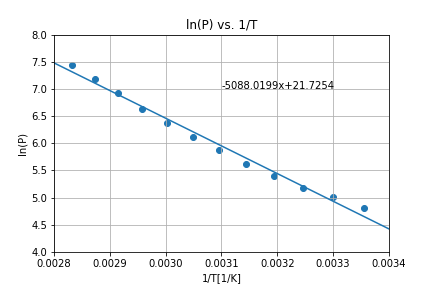
\includegraphics[scale=0.8]{mynd1.png}
    \caption{$\ln(p)$ sem fall af $1/T$. Hallatalan svarar til $-\Delta \widetilde{H}_{sub}/R$}
    \label{fig:mynd1}
\end{figure}

\begin{figure}[H]
    \centering
    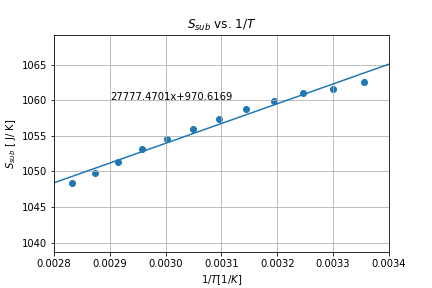
\includegraphics[scale=0.8]{mynd2.png}
    \caption{$S_{sub}$ sem fall af $1/T$. Hallatalan svarar til $\Delta \widetilde{H}_{sub}$}
    \label{fig:mynd2}
\end{figure}

Út frá mynd \ref{fig:mynd1} fáum við að $\Delta \widetilde{H}_{sub}^{(1)}/R = \SI{5088}{K}$ sem gefur okkur $\Delta \widetilde{H}^{(1)}_{sub} = \SI{42304}{J\per\mol}$\\

Út frá mynd \ref{fig:mynd2} fáum við að $\Delta \widetilde{H}^{(2)}_{sub} = \SI{27778}{J\per\mol}$\\

Við fáum því tvö tiltölulega ólík gildi fyrir $\Delta \widetilde{H}^{(i)}_{sub}$, en skekkjan er um $\sim 34\%$. Þetta má líklega útskýra með ónákvæmni í mælingum og gömlum mælibúnaði. Reynt var að nota mæligögn frá öðrum hópi en niðurstöðurnar sem fengust þar voru $\Delta \widetilde{H}^{(1')}_{sub} = \SI{32841}{J\per\mol}$ og $\Delta \widetilde{H}^{(2')}_{sub} = \SI{47350}{J\per\mol}$. Ástæða misræmis í þessum mismunandi niðurstöðum má mögulega rekja til ónákvæmni í framkvæmd, hitabaðið sem mæliglasið var í var óþétt og gæti hafa safnast vatnsgufa á hliðum mæliglassins. Þau gögn ásamt python kóða sem notuð voru í úrvinnslu þessarar tilraunar má nálgast á slóðinni \hyperlink{https://github.com/EmilGauti/dryodine}{github.com/EmilGauti/dryodine}.



\end{document}
